\normalfalse \difficiletrue \tdifficilefalse
\correctionfalse

%\UPSTIidClasse{11} % 11 sup, 12 spé
%\newcommand{\UPSTIidClasse}{12}

\exer{Résistance équivalente $\star$ \label{C1:06:538}}

\setcounter{numques}{0}
\UPSTIcompetence[2]{C1-06}
\index{Compétence C1-06}
\index{Grandeurs électriques}
\index{Lois de Kirchhoff}
\ifcorrection
\else
\textbf{Pas de corrigé pour cet exercice.}
\fi

\ifprof
\else

\question{Déterminer la résistance équivalente du dipole suivant.}
\begin{center}
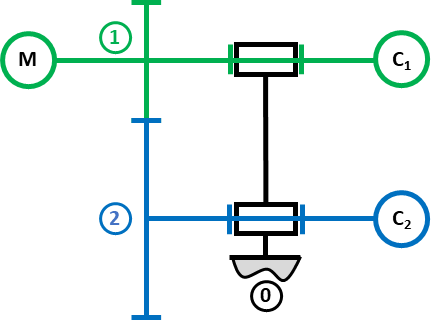
\includegraphics[width=\linewidth]{538_01}
\end{center}

\question{Déterminer le courant et la tension dans chacune des branches.}


\ifprof
\else
\begin{flushright}
\footnotesize{Corrigé  voir \ref{C1:06:538}.}
\end{flushright}%
\fi